\documentclass[./main.tex]{subfiles}
\graphicspath{{\subfix{./Abbildungen/}}}

\begin{document}
\renewcommand{\tasktitle}{Test OC Synthese}
\renewcommand{\taskpoints}{5}
\renewcommand{\taskweight}{7.9}
\aufgabenanfang
\blindtext

\kasten{5cm}{
    Antwort \punkte{5}
}{}

% \begin{center}    
% \begin{tabular}{ccc}
%     \begin{minipage}[c]{3cm}
%         \kasten{2cm}{\textbf{A}\par\begin{center}abc\end{center}}{}
%     \end{minipage} &
%     \begin{minipage}[c]{3cm}
%         \kasten{2cm}{\textbf{B}\\def}{}
%     \end{minipage}&
%     \begin{minipage}[c]{3cm}
%         \kasten{2cm}{\textbf{C}\\ghi}{}
%     \end{minipage}\\
% \end{tabular}
% \end{center}

\begin{center}
\tcbset{
  width=3.0cm + 6.3pt,
  colframe=black,
  colback=white,
  boxrule=0.4pt,
  arc=0pt,
  halign=left,
  boxsep=3pt,
  left=0pt,
  right=0pt,
  top=0pt,
  bottom=0pt,
}
\begin{tabular}{ccc}
    \begin{tcolorbox}
    \begin{minipage}[t][2cm][t]{3cm}
        \opt{1,2}{\textbf{A}\par\centering abc}\opt{0}{\textbf{A}}
    \end{minipage}
    \end{tcolorbox} 
    \hspace{0.5cm} &
    \begin{tcolorbox}
    \begin{minipage}[t][2cm][t]{3cm}
        \opt{1,2}{\textbf{B}\par\centering def}\opt{0}{\textbf{B}}
    \end{minipage}
    \end{tcolorbox} 
    \hspace{0.5cm} &
    \begin{tcolorbox}
    \begin{minipage}[t][2cm][t]{3cm}
        \opt{1,2}{\textbf{C}\par\centering ghi}\opt{0}{\textbf{C}}
    \end{minipage}
    \end{tcolorbox} \\
\end{tabular}
\end{center}


% TODO:
% include \opt{}
\kastenarray{6cm}{4cm}[0.5cm]{Q,W}{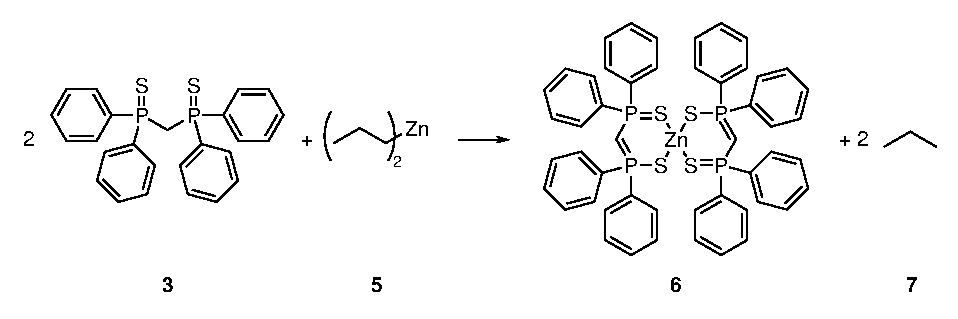
\includegraphics[width=5.5cm]{Komplex.eps},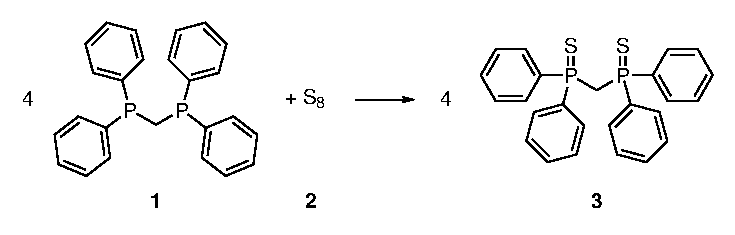
\includegraphics[width=5.5cm]{Ligand.eps}}

\kastenarray{2.5cm}{3cm}[0.3cm]{G,J,I,W}{1234,6425,672,6489}

Hier ein Text. 

\kastenarray{7cm}{7cm}[-0.44cm]{1,2}{Molekuel1,Molekuel2}

\textcolor{orange}{Zwei K\"asten direkt untereinander scheinen nicht zu funktionieren. Und auch die Musterl\"osung ist noch nicht integriert.}

\kastenarray{7cm}{7cm}[-0.44cm]{3,4}{Molekuel3,Molekuel4}


Hier ein Text. 

\clearpage
\aufgabenende
\end{document}